\documentclass{article}
\usepackage[polish]{babel}
\usepackage[T1]{fontenc}
\usepackage[utf8]{inputenc}
\usepackage{graphicx}
\usepackage{float}
\usepackage[bottom=1.5cm, right=2.5cm, left=2.5cm, top=1.5cm]{geometry}
\graphicspath{{../pliki}}



\title{%
  Cyberbezpieczeństwo - laboratoria 9 \\
  \large Ochrona komunikacji}
\author{Patryk Łuszczek 272707}
\date{\today}
\begin{document}
\maketitle
\newpage


\section*{Konfiguracja}

\begin{itemize}
  \item eth0:
        \begin{itemize}
          \item Kali Server: 10.0.4.4
          \item Ubuntu1 Client: 10.0.4.5
          \item Ubuntu2 Client: 10.0.4.6
        \end{itemize}
  \item tun0:
        \begin{itemize}
          \item Kali Server: 10.88.88.0
          \item Ubuntu1 Client: 10.88.88.6
          \item Ubuntu2 Client: 10.88.88.10
        \end{itemize}
\end{itemize}


\begin{figure}[H]
  \centering
  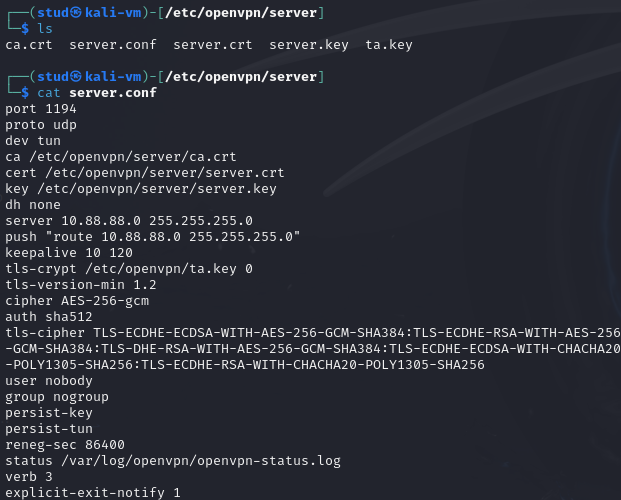
\includegraphics[width=0.8\textwidth]{1_zawartosc_serverconf.png}
  \caption{Serverconf}
\end{figure}


\section{TLS}
Przechwytywanie ruchu sieciowego
\begin{figure}[H]
  \centering
  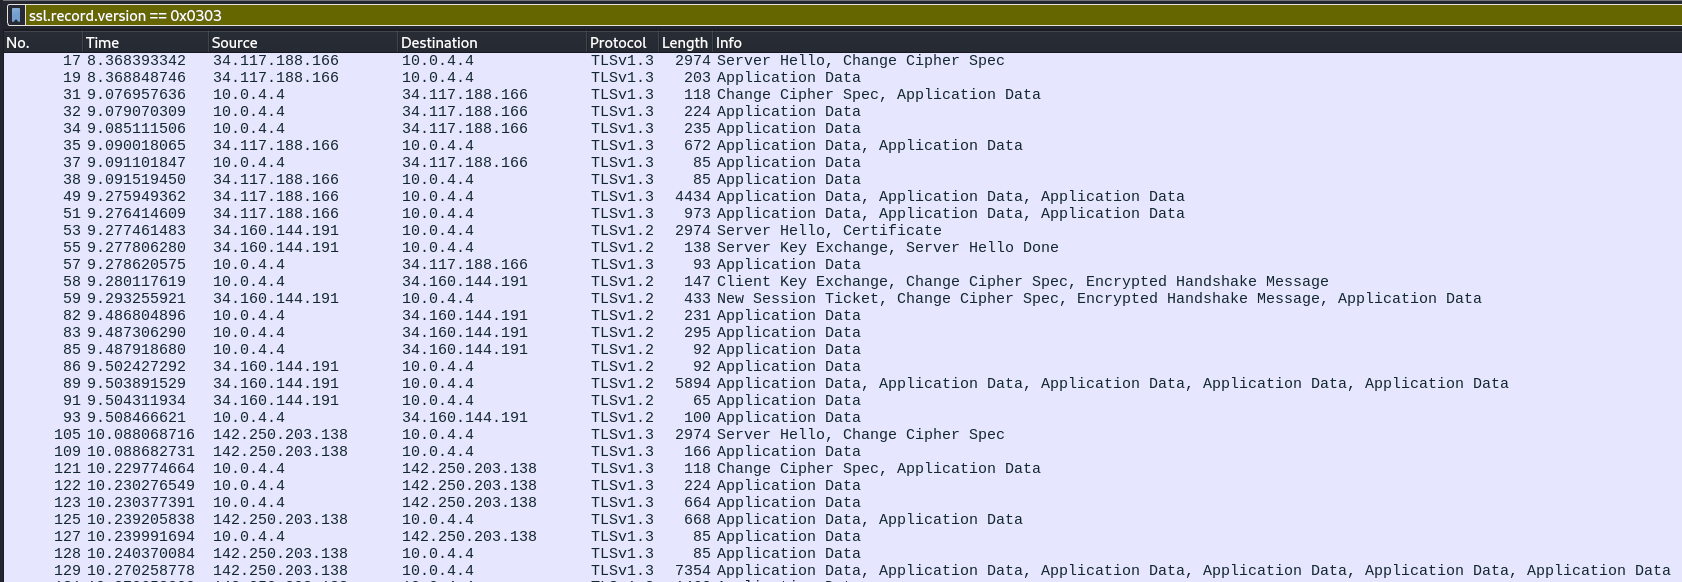
\includegraphics[width=0.8\textwidth]{4_filtrtslssl.png}
  \caption{Wireshark}
\end{figure}
\subsection*{1.3}
\begin{figure}[H]
  \centering
  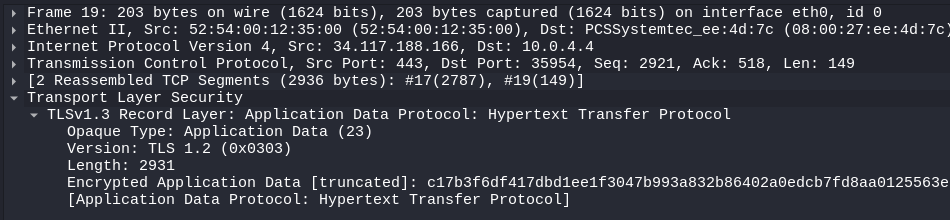
\includegraphics[width=0.8\textwidth]{5_przykladtsl.png}
  \caption{Ramka handshake}
\end{figure}
\begin{figure}[H]
  \centering
  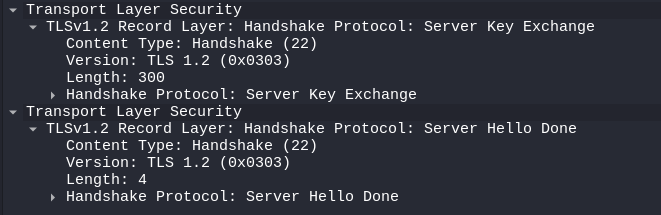
\includegraphics[width=0.8\textwidth]{5_przykladtsl2.png}
  \caption{Przykładowa ramka}
\end{figure}
\begin{figure}[H]
  \centering
  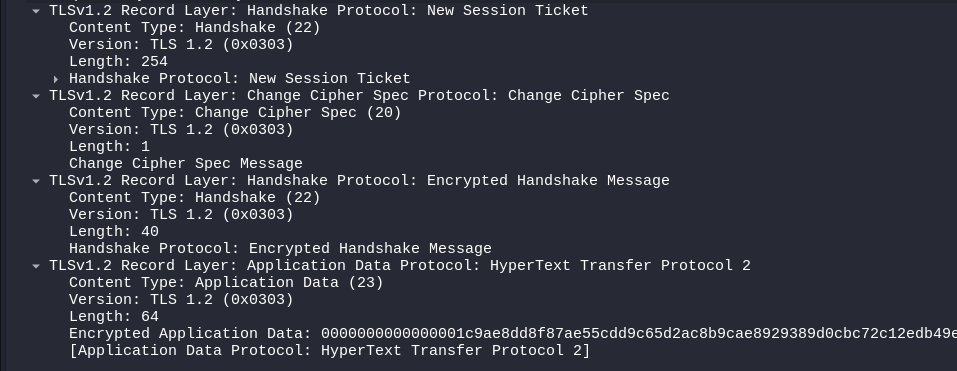
\includegraphics[width=0.8\textwidth]{5_przykladtslwiecej.png}
  \caption{Przykładowa ramka}
\end{figure}
\begin{figure}[H]
  \centering
  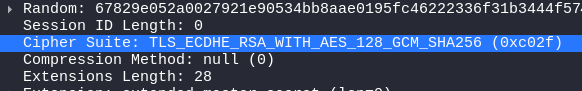
\includegraphics[width=0.8\textwidth]{6_tls2_szyfr.png}
  \caption{Szyfr tsl2}
\end{figure}
\begin{figure}[H]
  \centering
  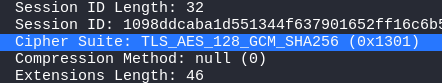
\includegraphics[width=0.8\textwidth]{6_tls3_szyfr.png}
  \caption{Szyfr tsl1}
\end{figure}

Przechwycono następujące typy rekordów:
\begin{itemize}
  \item Server Hello
  \item Change Cipher Spec
  \item Application Data
  \item Server Key Exchange
  \item Server Hello done
  \item Client Key Exchange
  \item Encrypted Handshake Message
\end{itemize}
\subsection*{1.4 Czy TLS i SSL to ten sam protokół?}
TLS i SSL to zasadniczo ten sam protokół, jednakże TLS jest ulepszeniem SSL naprawiającym jego luki w zabezpieczeniach.
\subsection*{1.5 Co to jest TLS/SSL handshake?}
Handshake to proces wymiany kluczy i ustalania parametrów bezpieczeństwa zanim rozpoczie się właściwa komunikacja.
\subsection*{1.6 Co zapewnia protokół TLS/SSL, podaj przykłady jego zastosowań (przynajmniej
  2)?}
Protokół zapewnia ochronę transmisji poszczególnych danych przez ich szyfrowanie oraz zastosowanie procesu uwierzytelniania (certyfikaty)
\begin{itemize}
  \item Szyfrowanie komunikacji w internecie na stronach zabezpieczonych protokołem HTTPS (np. logowanie do banku)
  \item Szyfrowanie komunikacji e-mail - zabezpieczenie komunikacji pomiędzy serwerem poczty a klientem
\end{itemize}
\subsection*{1.7 Które wersje protokołu są obecnie najpopularniejsze?}
Obecnie najpopularniejsza jest wersja TLS 1.3. Oprócz niej wciąż stosowana jest werja TLS 1.2. Starsze wersje są uważane za przestarzałe.
\subsection*{1.8 Która wersja zapewnia większe bezpieczeństwo i dlaczego?}
Największe bezpieczeństwo zapewnia wersja 1.3. W wersji 1.3 są używanie jedynie algorytmy szyfrowania, które obecnie nie mają znanych słabości. Usunięto również opcję "renegocjacji", która była podatna na ataki.
\subsection*{1.9 Która wersja zapewnia wyższą wydajność?}
Większą wydajność zapewnia wersja 1.3. Usprawniony został proces handshake.
\subsection*{1.10 Która wersja protokołu została przechwycona?}
Obydwie wersje 1.2 i 1.3 zostały przechwycone.
\subsection*{1.11 Z jakiego rodzaju wiadomości składa się uzgadnianie (nawiązanie
  połączenia)?}
Uzgadnianie połączenia składa się z następujących wiadomości:
\begin{itemize}
  \item Client Hello - klient wysyła zgłoszenie zawierające informacje o m.in obsługiwanej wersji SSL, dozwolonych sposobach szyfrowania
  \item Server Hello - klient zwraca wybrane parametry
  \item Certificate - serwer wysyła swój certyfikat
  \item Server Key Exchange - serwer wysyła informacje o swoim kluczu publicznym
  \item ServerHelloDone - serwer informuje, że może przejść do następnej fazy
  \item ClientKeyExchange - klient wysyła wstępny klucz sesji
  \item ChangeCipherSpec - klient/serwer informjue, że od tej pory będzie wysyłał tylko zaszyfrowane informacje
  \item Finished - komunikat o pomyślnym procesie handshake wysłany bezpiecznym kanałem
\end{itemize}
\subsection*{1.12 Od czego zależy wersja używanego protokołu?}
Wersja zależy od konfiguracji serwera i klienta oraz od wyniku negocjaji.

\section{OpenVPN - przesył przez VPN}

\begin{figure}[H]
  \centering
  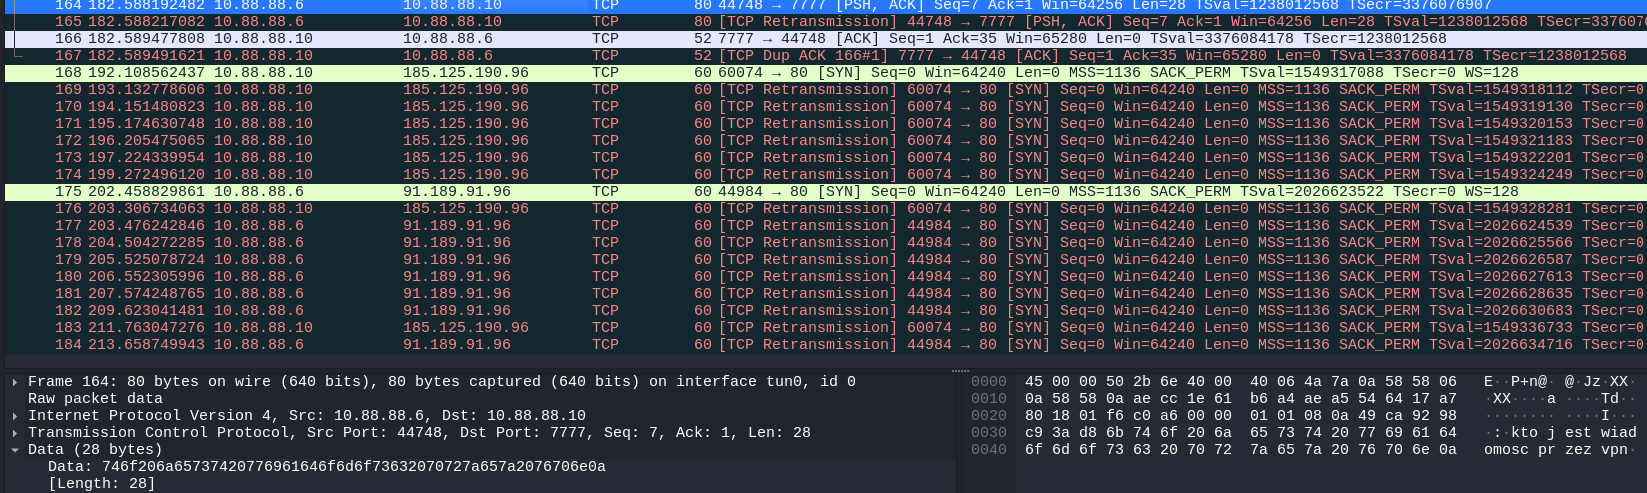
\includegraphics[width=0.8\textwidth]{8_netcat_tun0.png}
  \caption{Ramka przesłana przez tun0}
\end{figure}

Jak można zauważyć wiadomość wysłana pomiędzy klientami jest możliwa do odczytania w programie Wireshark.

\section{OpenVPN - przesył przez eth0}
\begin{figure}[H]
  \centering
  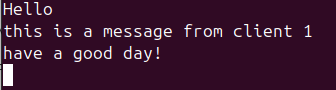
\includegraphics[width=0.8\textwidth]{7_wyslanewiadomosci.png}
  \caption{Odebrana wiadomość}
\end{figure}
\begin{figure}[H]
  \centering
  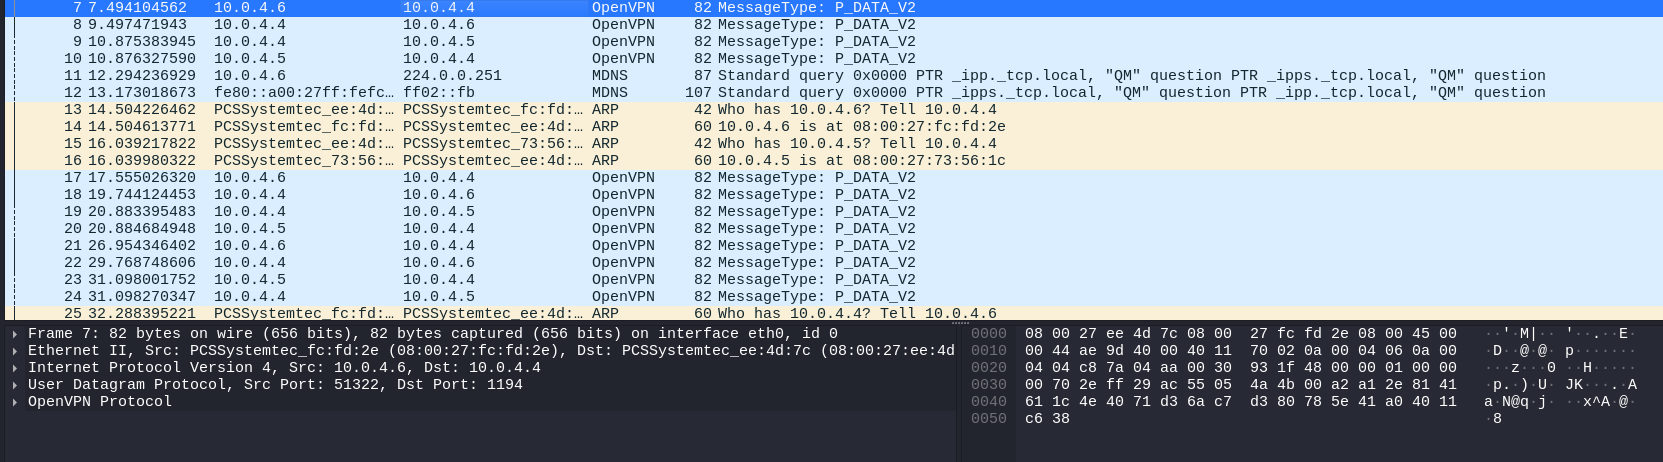
\includegraphics[width=0.8\textwidth]{8_netcat_eth0.png}
  \caption{Ramka przesłana przez eth0}
\end{figure}


\subsection*{3.5 Czy można odczytać wiadomość wysłaną przez netcat?}
W przypadku przesyłania wiadomości przez interfejs fizyczny było widać pakiety OpenVPn, którego dane miały zaszyfrowaną postać - więc były niemożliwe do odczytania.
Wiadomość przesłana przez interfejs VPN (tun0) była możliwa do odczytania.
\subsection*{3.6 Jaka jest charakterystyka przechwyconego ruchu na interfejsie sieci VPN i
  interfejsie hosta?}
W przypadku ruchu na interfejsie VPN pakiety przechodziły bezpośrednio z adresu źródła do klienta docelowego.
W przypadku ruchu na interfejsie fizycznym pakiety pierw przechodziły przez serwer a dopiero później z serwera zostały przesyłane do klienta docelowego.

\subsection*{3.7 Jakie istotne informacje można zobaczyć analizując ruch w obu przypadkach?}
Dla ruchu w sieci VPN można zobaczyć jawny tekst przesłanej wiadomości, która jest zaszyfrowana dla ruchu na interfejsie fizycznym.
\section{Przesyłanie dużego pliku}
\begin{table}[H]
  \centering
  \begin{tabular}{|c|c|c|}
    \hline
    Cipher      & Auth   & Time  \\
    \hline
    AES-256-GCM & SHA512 & 29s   \\
    \hline
    AES-128-CBC & SHA1   & 38s   \\
    \hline
    DES-EDE-CBC & MD5    & 36s   \\
    \hline
    DES-CBC     & MD5    & błąd* \\
    \hline
  \end{tabular}
  \caption{Czasy przesyłania dużego pliku}
\end{table}

\begin{figure}[H]
  \centering
  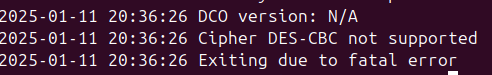
\includegraphics[width=0.8\textwidth]{10_notsupported.png}
  \caption{Błąd dla konfiguracji 4}
\end{figure}

\begin{figure}[H]
  \centering
  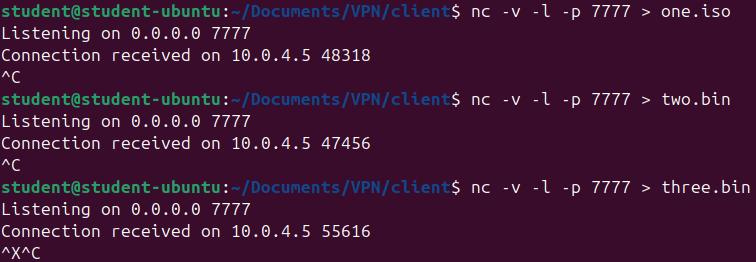
\includegraphics[width=0.8\textwidth]{recieved files.png}
  \caption{Odbieranie dużych plików}
\end{figure}
\subsection*{4.4 Czy istnieje różnica w czasach przesyłania danych? Co może na nich wpłynąć?}
Istnieje niewielka różnica w czasie przesyłu danych. Na te różnice możne wpływnąc zastosowanie mniej lub bardziej wydajnego czasowo algorytmu szyfrowania.
\subsection*{4.5 Co możemy powiedzieć o zastosowanych algorytmach szyfrowania i
  uwierzytelniania?}

Algorytm AES-256-GCM jest jest najsilniejszym spośród użytych algorytmów, jest powszechnie stosowany do szyfrowania danych i jest uznawany za bezpieczny. Algorytm
AES-128-CBC jest nieco mniej bezpieczny niż poprzedni algorytm, przede wszystkim ze względu na mniejszy klucz. Algorytm DES-EDE-CBC jest uznawany za bezpieczny, jednak zaleca się wykorzystywanie AES.
Algorytm uwierzytelniania SHA512 używa klucza długości 512-bit i jest uznawany za bardzo bezpieczny. SHA1 ma klucz długości 160-bit i jest mniej bezpieczny niż wersja 512-bitowa. Algorytm MD5 nie jest już uważany za bezpieczny i zaleca się używanie algorytmów SHA.


\subsection*{4.6 Który zestaw ustawień jest najgorszy, a który najlepszy pod względem
  bezpieczeństwa?}

Najmniej bezpieczne jest zestawienie DES-CBC wraz z MD5. Są to już nieużywanie powszechnie algorytmy, ponieważ znane są metody skutecznych ataków na nie.
Najbezpieczniejszy zestaw to użycie algorytmu AES-256-GCM w połączeniu z uwierzytelnianiem SHA512. Użyte długości kluczy w obu algorytmach są wystarczająco długie, aby zagwarantować bezpieczeństwo.


\end{document}